%
% Tesi D.S.I. - modello preso da
% Stanford University PhD thesis style -- modifications to the report style
%
%%%%%%%%%%%%%%%%%%%%%%%%%%%%%%%%%%%%%%%%%%%%%%%%%%%%%%%%%%%%%%%%%%%%%%%%%%%
%                                                                         %
%			TESI DOTTORATO                                                %
%			______________                                                %
%                                                                         %
%			AUTORE: Andrei Ciulpan                                        %
%                                                                         %
%			Ultima revisione: 5.05.2019                                  %
%                                                                         %
%%%%%%%%%%%%%%%%%%%%%%%%%%%%%%%%%%%%%%%%%%%%%%%%%%%%%%%%%%%%%%%%%%%%%%%%%%%
%
%
\documentclass[12pt]{report}
%    \renewcommand{\baselinestretch}{1.6}      % interline spacing
%
% \includeonly{}
%
%			PREAMBOLO
%
\usepackage[a4paper]{geometry}
\usepackage{amssymb,amsmath,amsthm}
\usepackage{graphicx}
\usepackage[hyphens,spaces,obeyspaces]{url}
\usepackage{hyperref}
\usepackage{epsfig}
\usepackage[italian]{babel}
\usepackage{tesi}
\usepackage{afterpage}

\addto{\captionsitalian}{%
	\renewcommand{\bibname}{Sitografia}
}

\newcommand\blankpage{%
	\null
	\thispagestyle{empty}%
	\addtocounter{page}{-1}%
	\newpage}

% per le accentate
\usepackage[utf8]{inputenc}
%
\newtheorem{myteor}{Teorema}[section]
%
\newenvironment{teor}{\begin{myteor}\sl}{\end{myteor}}
%
%
%			TITOLO
%
\begin{document}
\title{Sistema Accessi IoT}
\author{Andrei CIULPAN}
\dept{Corso di Laurea in Informatica} 
\anno{2018/2019}
\matricola{872394}
\relatore{Dott. Andrea TRENTINI}
\correlatore{Marco LANZA}
\afterpage{\blankpage}
% 
%			DEDICA
%
\beforepreface

{\hfill \footnotesize {\sl Ringrazio i miei genitori e la nonna per il sostegno e per la pazienza che hanno avuto.}}
\vskip 0.8cm
{\hfill \footnotesize {\sl Ringrazio i miei amici e compagni di università per aver reso l'esperienza più bella e soprattutto più facile.}}
\vskip 0.8cm
{\hfill \footnotesize {\sl Ringrazio i miei tutor e colleghi per avermi dato la possibilità di crescere e concludere la mia esperienza universitaria.}}
\vskip 0.8cm
{\hfill \footnotesize {\sl Un ringraziamento speciale a Elena per essere riuscita a farmi sorridere e a tirarmi su il morale in ogni giorno con la sua presenza nella mia vita.  Un altro ringraziamento a lei per la revisione della tesi.}}
       

\afterpreface

% 
%			CAPITOLO 1: Intro
\chapter{Introduzione}\label{cap:introduzione}
%

Il controllo accessi è un sistema di protezione che permette l'accesso solo a determinate persone per via di qualche procedura di autenticazione: nel mondo fisico si può parlare di una semplice serratura (storicamente il sistema piu' utilizzato in assoluto) che può essere aperta solo dalle persone in possesso della chiave, mentre nel mondo dell'informatica si può notare l'enorme utilizzo delle procedure di autenticazione (login) che aiutano il sistema, tramite l'inserimento di un nome utente e password, a determinare automaticamente se una persona è autorizzata ad accedere alle risorse del sistema stesso.

Il controllo accessi\cite{controllo_accessi} è un tema molto sviluppato nel campo della sicurezza sia fisica che informatica: è stato segnalato che nel 2017, per il secondo anno consecutivo, il mercato del controllo accessi ha avuto la crescita piu' rapida nell'industria della sicurezza fisica\cite{crescita_controllo_accessi}. E' anche un sistema onnipresente, utilizzato in ospedali, fabbriche, supermercati, aziende, sistemi di trasporto pubblico (e.g l'ATM di Milano), case e tanti altri campi.  

La tesi si propone di trattare un sistema ibrido in cui il mondo fisico e il mondo informatico lavorano insieme: attraverso sensori ed attuatori è possibile avere la comunicazione tra i due mondi. 
Si tratta di un sistema IoT (Internet of Things), ovvero un sistema in cui la connessione Internet viene estesa anche al mondo degli oggetti fisici (smart objects\cite{smart_objects}) di uso comune. Gli oggetti si rendono riconoscibili e acquisiscono intelligenza grazie al fatto di possedere una o piu' delle seguenti funzionalità: identificazione, localizzazione, diagnosi di stato, interazione con l'ambiente circostante, elaborazione dati e ovviamente connessione.
Gli oggetti intelligenti di un sistema IoT sono normalmente dotati di un processore embedded, sensori e attuatori e sono in grado di agire sui dati raccolti dall'ambiente e, ancora piu' importante, mandare questi dati in rete dove possono poi essere analizzati\cite{IoT}. Un semplice esempio di un sistema IoT si può trovare in Figura 1.\marginpar{atrent: metti riferimenti con \\ref{key}, commento valido su tutto il testo}

Le seguente sezione di questo capitolo introdurrà il progetto stesso (denominato SimSim) che poi verrà dettagliato nei prossimi capitoli.

\begin{figure}
	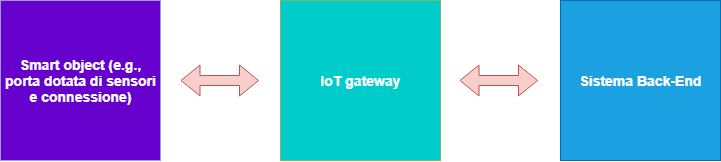
\includegraphics[width=\linewidth]{./img/iot_diagram.png}
	\caption{Esempio di sistema IoT}\label{fig:iot1}
\end{figure}

%
\section{Requisiti del progetto}
%

L'attività principale del tirocinio è la realizzazione di un sistema di controllo accessi, da applicare presso varchi. Vengono elencati i requisiti del sistema:

\begin{enumerate}
	\item Deve essere in grado di funzionare con diverse modalità di riconoscimento:
	\begin{enumerate}
		\item Tessera RFID
		\item Tastierino numerico (password)
		\item Telecomando RF 
	\end{enumerate}
	\item Deve dare la possibilità di visualizzare su un display LCD ciò che sta succedendo (accesso consentito/negato ecc...). Inoltre deve essere implementata una funzione che permetta di visualizzare i codici delle tessere RFID sul display LCD (operazione protetta da una password).
	\item A seguito di ogni accesso avvenuto con successo deve aprire una porta (usando un servomotore) e salvare il log in un database remoto (in LAN) tramite WiFi.
	\item Deve avere un database per:
	\begin{enumerate}
		\item Tessere RFID
		\item Log degli accessi
		\item Soci
	\end{enumerate}
	\item Deve avere un'interfaccia grafica (in questo caso sito web) tramite la quale l'utente amministratore possa gestire il database con le seguenti funzioni: \begin{enumerate}
		\item Aggiungere/modificare/cancellare soci 
		\item Aggiungere/modificare/cancellare tessere 
		\item Visualizzare log
	\end{enumerate}
\end{enumerate}

I dispositivi scelti per soddisfare i requisiti sono stati un Arduino UNO (per la parte hardware) e un Raspberry Pi 3B+ su cui hostare il server. 
Nella figura 2 si può vedere una foto con il prototipo finito.
Nelle figure 3 e 4 si possono trovare rispettivamente un diagramma dei casi d'uso e un diagramma di flusso del sistema.


\begin{figure}
	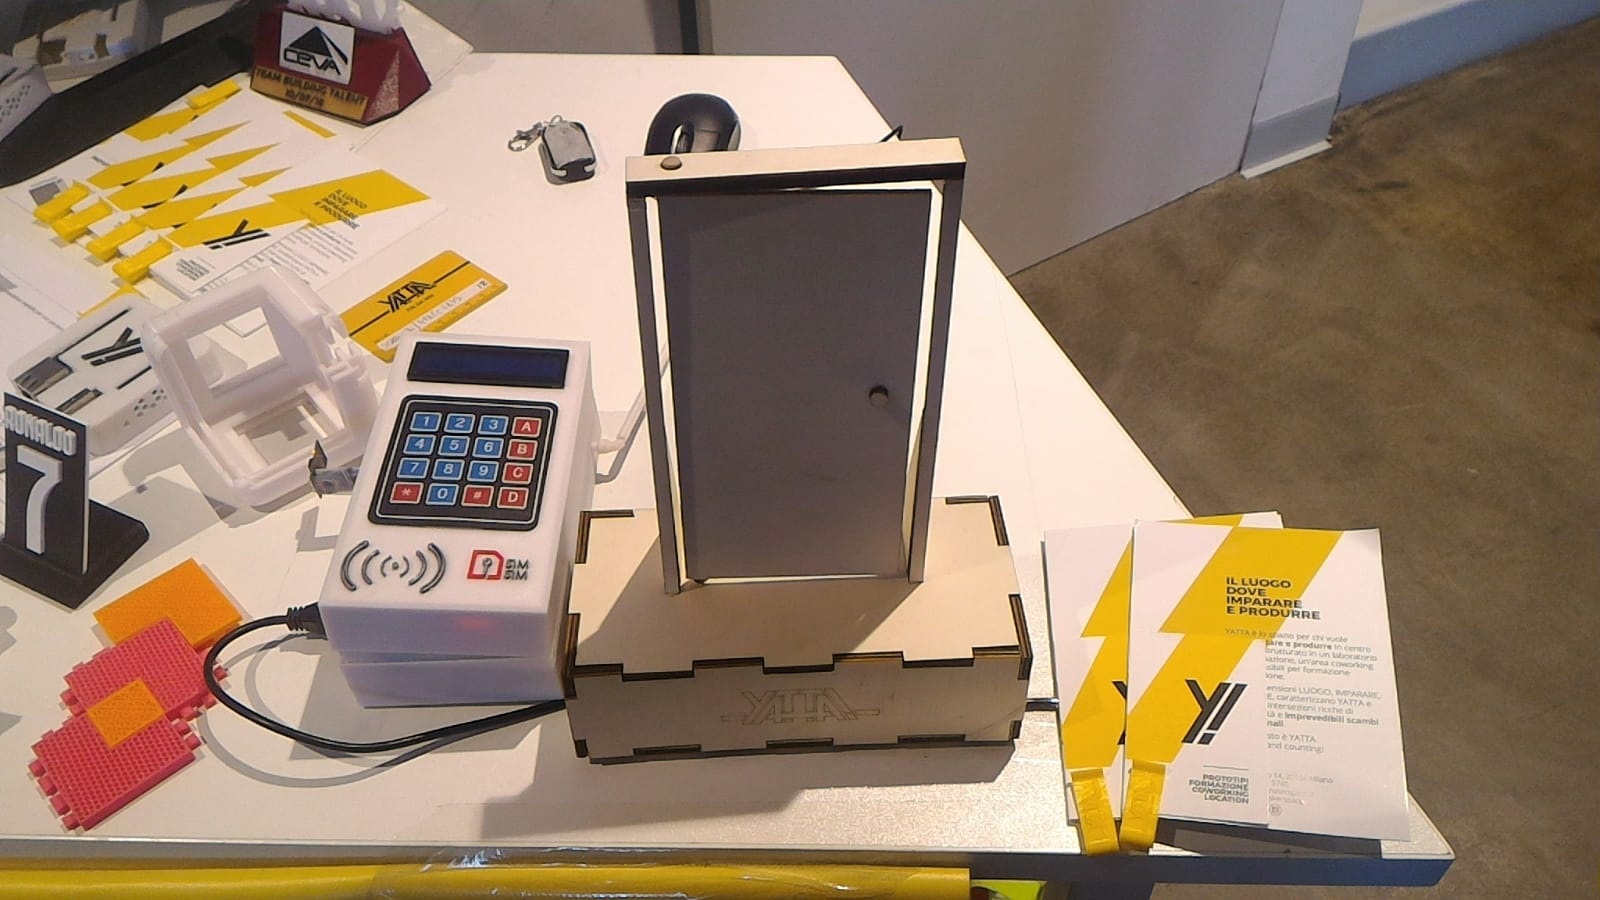
\includegraphics[width=1\linewidth]{./img/simsim.jpeg}
	\caption{SimSim}
	\label{fig:flux}
\end{figure}

\begin{figure}
	\center{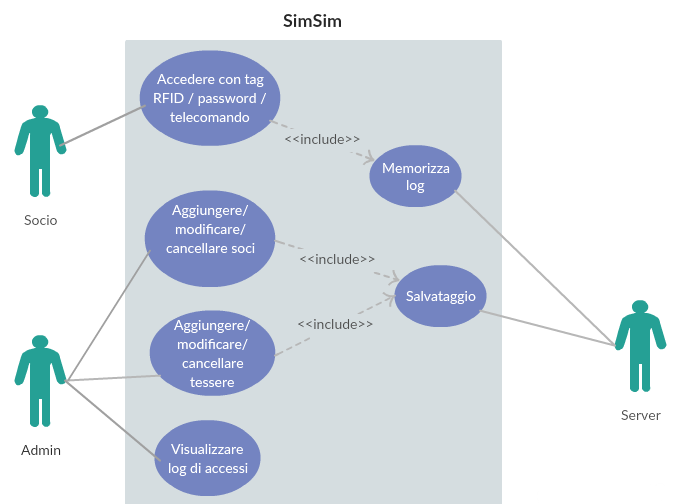
\includegraphics[width=0.6\linewidth]{./img/usecase.png}}
	\caption{Casi d'uso del sistema}
	\label{fig:usecase}
\end{figure}

\begin{figure}
	\center{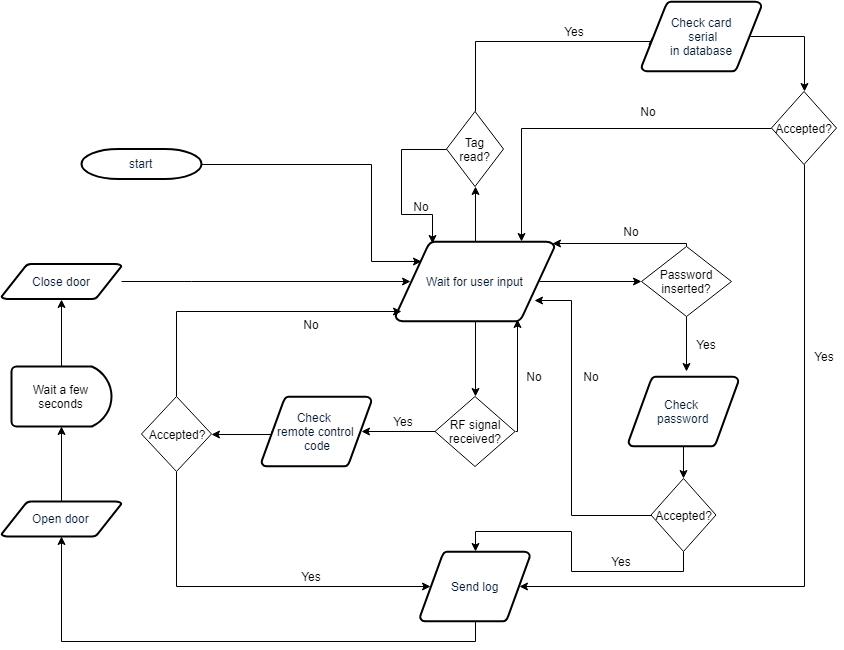
\includegraphics[width=0.9\linewidth]{./img/flowchart.png}}
	\caption{Diagramma di flusso del sistema}
	\label{fig:usecase}
\end{figure}



%			CAPITOLO 2: Hardware
\chapter{Hardware}
\label{cap2}
%

In questo capitolo vengono dettagliati i dispositivi hardware utilizzati nel progetto. Uno schema completo del circuito elettrico si trova in Figura 5.

\begin{figure}
	\center{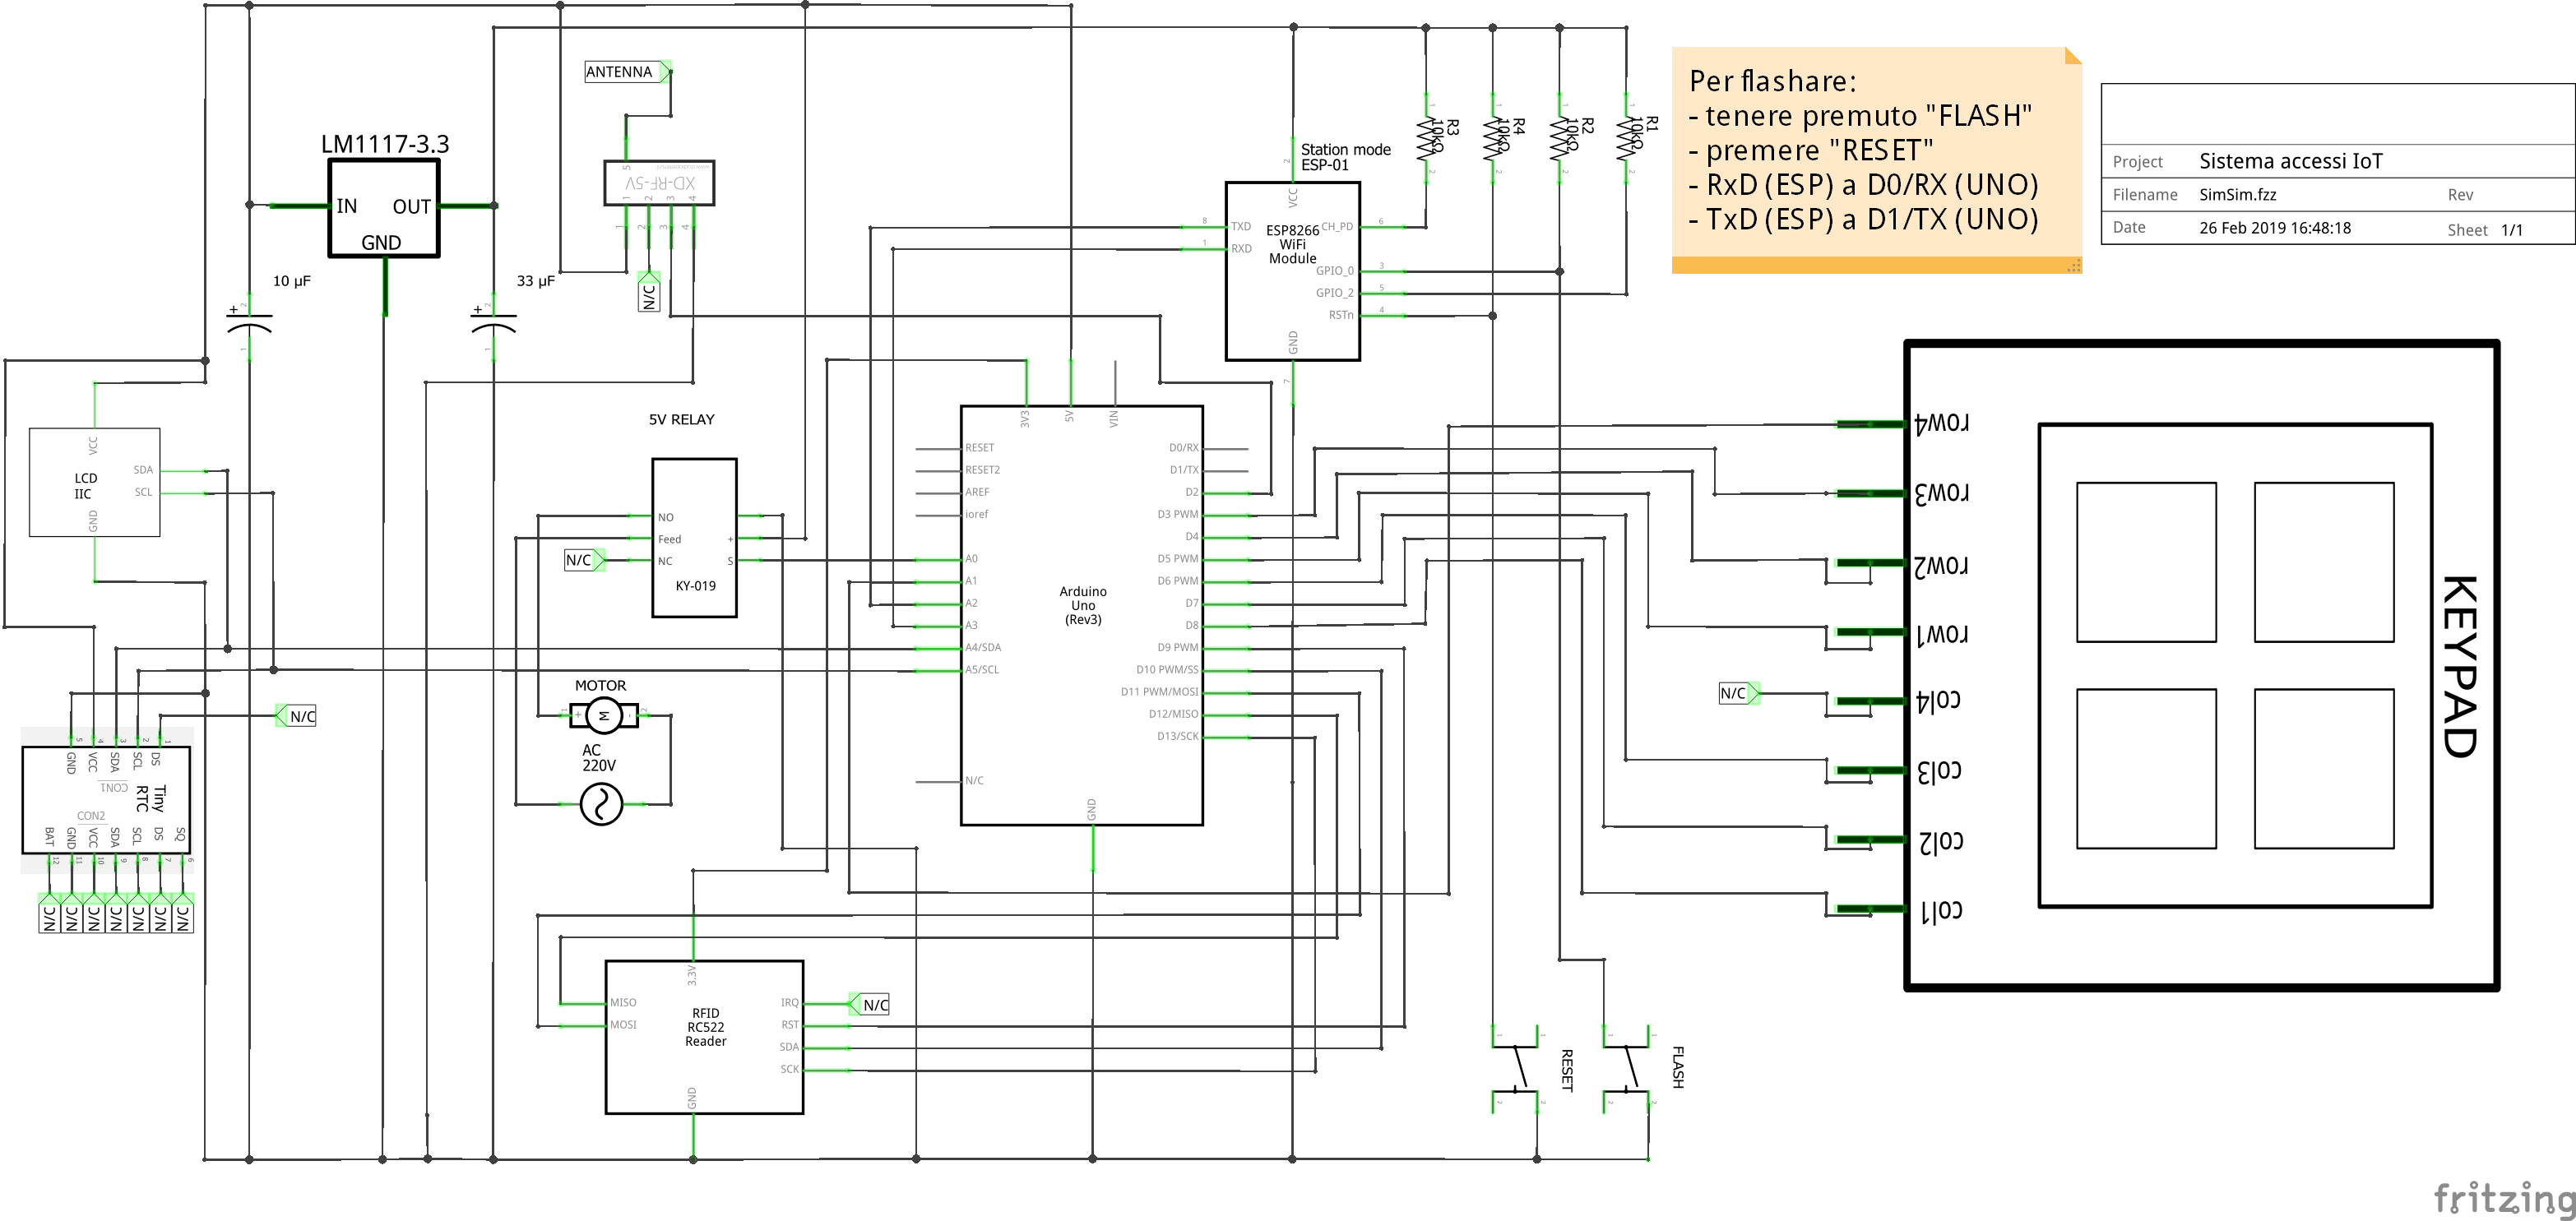
\includegraphics[width=\textwidth,height=1.1\textheight,keepaspectratio]{./img/schematics.png}}
	\caption{Schema del circuito}
	\label{fig:flux}
\end{figure}


%

\section{Raspberry Pi}
%

Raspberry Pi (Figura 6) è una serie di piccoli computer (system-on-chip) dalle dimensioni simili a quelle di una carta di credito. La scheda è stata sviluppata nel Regno Unito (Fondazione Raspberry Pi). Le prime versioni avevano poca potenza computazionale e sono state progettate con l'intenzione di offrire a insegnanti e studenti uno strumento semplice e poco costoso con cui poter insegnare e imparare a programmare. La scheda ha avuto un enorme successo anche in altri campi (e.g. robotica) e con ogni nuova versione è stata migliorata. Le ultime versioni sono assai potenti e possono essere utilizzati per tante altre cose. Le schede sono basate su sistemi operativi di tipo GNU/Linux, in particolare Raspbian che può essere scaricato dal sito della fondazione (\url{https://www.raspberrypi.org/downloads/}). 

La scheda utilizzata nel progetto (Raspberry Pi 3B+, \url{https://www.raspberrypi.org/products/raspberry-pi-3-model-b-plus/}) possiede un'architettura su 64 bit, essenziale per poter utilizzare in maniera efficiente MongoDB (che è limitato a una memoria di 2GB su un sistema a 32bit). Durante lo sviluppo del progetto ho scoperto che Raspbian in realtà non è stato ancora aggiornato per essere un sistema operativo a 64 bit, perciò non poteva sfruttare al meglio la scheda. Come soluzione a questo problema, è stato installato un sistema operativo chiamato openSUSE Tumbleweed (\url{https://software.opensuse.org/distributions/tumbleweed}) che funziona su architetture a 64 bit. 
La Raspberry Pi 3B+ possiede inoltre una scheda WiFi, il che la rende un buon candidato per lo scopo principale del progetto, ovvero quello di hostare il server.

\begin{figure}
	\center{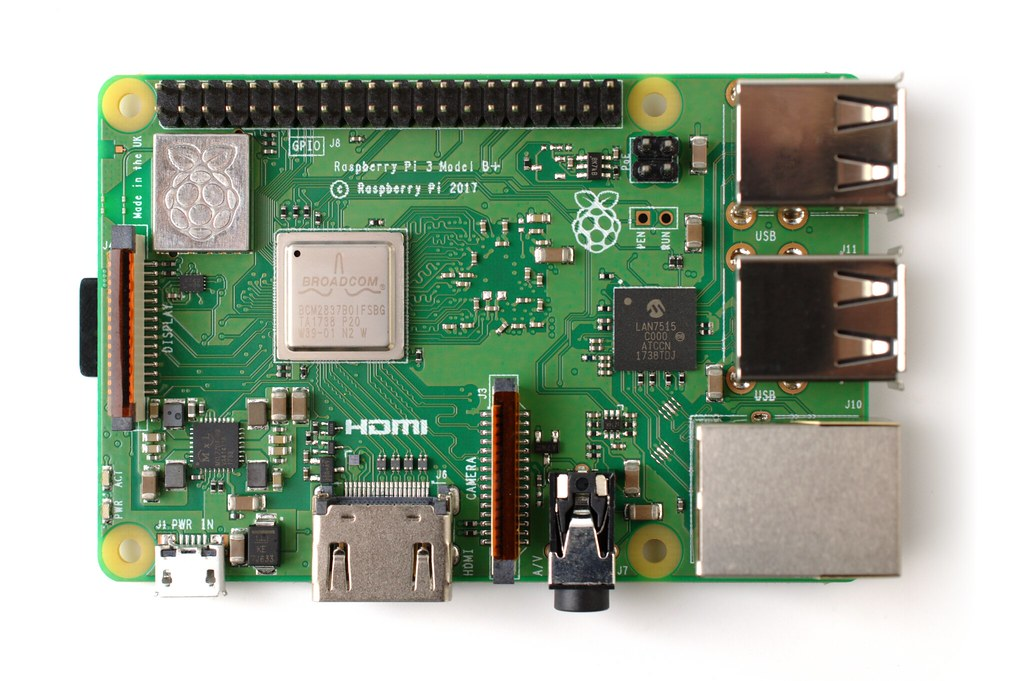
\includegraphics[width=0.4\linewidth]{./img/raspi.jpg}}
	\caption{Scheda Raspberry Pi}
	\label{fig:usecase}
\end{figure}


\section{Arduino UNO}
%

Arduino\cite{arduino_storia} è nata ad Ivrea nel 2005 come piattaforma di prototipazione elettronica di basso costo e open-source (dettaglio molto importante che ha portato al successo che ha avuto) che si basa su hardware e software flessibili e facili da usare. Il nome della scheda deriva di quello del bar di Ivrea frequentato dai fondatori del progetto ed la scheda è stata creata per artisti, designer e hobbisti. Essendo open-source, ha avuto un grande successo nel mondo degli hobbisti, anche a livello mondiale (tale da diventare una delle invenzioni piu' considerevoli nella storia dell'elettronica), grazie alla facilità di programmazione, basso costo e soprattutto disponibilità in rete delle informazioni necessarie per poter permettere a persone con grandi idee e poche capacità informatiche ed elettroniche di realizzare i propri progetti. 

Nei giorni d'oggi Arduino potrebbe anche non essere la scelta immediata, anzi, ormai ci sono schede piu' potenti, piu' veloci e con migliori rapporti prestazioni/prezzo, ma non scordiamoci che è tutto grazie agli sviluppatori della scheda. Perchè scegliere, quindi, un Arduino? Essendo la scheda che ha fatto partire tutto, è anche la scheda piu' studiata e ciò significa che gira intorno a piu' informazioni, piu' librerie già pronte, piu' dispositivi compatibili e ha anche un sito di appassionati che si aiutano a vicenda dove si possono trovare tutorial, libri e tant'altro.

La scheda utilizzata nel progetto, Arduino UNO (Figura 7), è assolutamente la scheda piu' conosciuta al mondo e si può ormai trovare a dei prezzi molto bassi (ci sono tanti clone diversi in rete grazie al fatto di essere OpenHardware). E' basato sul microcontrollore ATmega328P (\url{https://www.sparkfun.com/datasheets/Components/SMD/ATMega328.pdf}) ed ha 14 pin digitali e 6 analogici. Alcuni pin sono piu' speciali: ad esempio tra i pin digitali ci sono 6 che hanno anche la funzione PWM (si veda la sezione 2.5 "Servomotore") e 4 per il protocollo SPI (si veda la sezione 2.10.4 "SPI"), mentre tra i pin analogici ci sono 2 per il protocollo I2C (si veda la sezione 2.10.3 "I2C"). Tutto questo rende l'Arduino UNO un dispositivo ideale per il progetto. L'unica cosa che manca è la possibilità di accedere alla connessione WiFi, indispensabile per l'IoT, ma questo problema è stato risolto grazie ad un chip WiFi chiamato ESP8266 (si veda la sezione 2.9 "ESP8266").

\begin{figure}
	\center{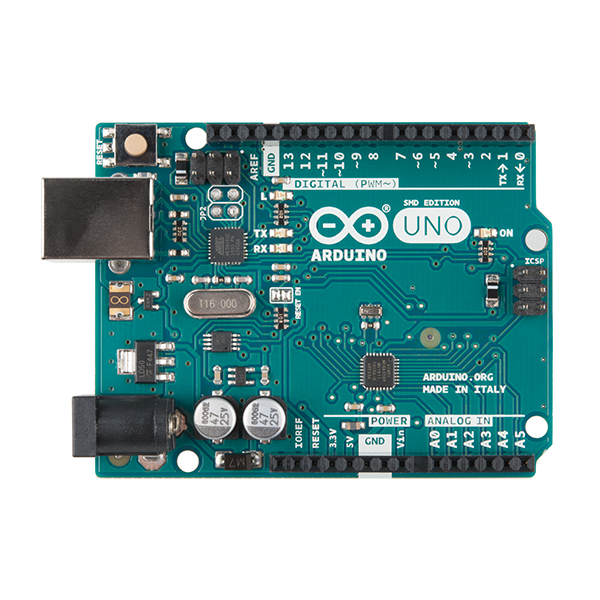
\includegraphics[width=0.4\linewidth]{./img/uno.jpg}}
	\caption{Scheda Arduino UNO}
	\label{fig:usecase}
\end{figure}


\subsection{Arduino Programming Language}

La scheda Arduino UNO (e qualsiasi altra board compatibile con Arduino) può essere facilmente programmata utilizzando, ma non solo, l'Arduino IDE (Arduino Integrated Development Software), un software sviluppato da Arduino.cc e funzionante sulle 3 piattaforme dominanti (Windows, Linux e MacOS). Il linguaggio di programmazione si chiama "Arduino Programming Language"\cite{sistemi_embedded_atrent} ed è un derivato di Wiring (una piattaforma di sviluppo open-source composta da un linguaggio di programmazione, un IDE ed un circuito stampato basato su un microcontrollore). La sintassi è molto simile a quella del linguaggio C/C++; infatti il linguaggio Arduino è un insieme di funzioni e librerie C/C++ che possono essere chiamate dal codice. Forse la cosa diversa che si nota di piu' è la struttura dello sketch (sinonimo di programma): per poter funzionare vengono sempre definite due funzioni iniziali, setup() e loop(); la prima viene eseguita soltanto una volta all'avvio del programma e serve per dichiarare variabili, modalità dei pin (e.g input o output) ecc., mentre nella seconda viene messo il programma vero e proprio che viene eseguito ripetutamente... all'infinito.

%
\section{RTC (perchè la Raspberry Pi non ce l'ha ed è privo di connessione Internet)}
%
\section{Ricevitore RF}
Un po' di matematica sulle antenne
%
\section{Servomotore}
PWM
\\ 
\section{RFID}
%
\section{Display LCD 16x2}
%
\section{Keypad}
%
\section{ESP8266}
%
Problematiche
\\
Alternative
\section{Protocolli di trasmissione dati}
\subsection{Logica IoT}
%
\subsection{Comunicazione Wi-Fi in rete locale. Parlo anche del protocollo HTTP?}
%
\subsection{I2C}
%
\subsection{SPI}
% 
%			CAPITOLO 3: Software
\chapter{Software}
\label{cap3}
%
%
%
\section{Strumenti dello sviluppatore}
Arduino IDE
\\
Node.js
\\
Postman
\\
MongoDB 
\\
Per i linguaggi di programmazione metto solo un riferimento alla bibliografia
%
%
\section{Sviluppo del sistema embedded}
Snippet e spiegazioni di codice
\\

%
%
\section{Sviluppo dell'interfaccia web}
%
\subsection{Back-End}
\subsection*{Scelte progettuali}
MVC
\subsection*{Database}
%
\subsection*{API}
Documentazione delle API del back-end
%
\subsection{Front-End}
\subsection*{Scelte progettuali}
Le basi: Javascript, HTML5 \& CSS
\\
w3.css
\\
jQuery
\\
EJS
\\
%
% 
%			CAPITOLO 4: Analisi del progetto
\chapter{Analisi del progetto}
\label{cap4}
Prestazioni
\\
Problema sicurezza
\\
Possibili miglioramenti
\\
%
% 
%			CAPITOLO 5: Conclusioni
\chapter{Conclusioni}


\label{cap5}
%
%

\appendix
\chapter{Una prima Appendice (?)}
...

%
%			BIBLIOGRAFIA
%
\begin{thebibliography}{00}
	

\bibitem{controllo_accessi}
J. Allen, Opening new doors with IP access control, 16 Marzo, 2018. \url{https://www.axis.com/blog/secure-insights/opening-new-doors-with-ip-access-control/}
%

\bibitem{crescita_controllo_accessi}
R. Alalouff, Access control leads growth in physical security market but video surveillance still dominates, 25 Gennaio, 2018.
\url{https://www.ifsecglobal.com/access-control/access-control-leads-growth-physical-security-market-video-surveillance-still-dominates/}
%
\bibitem{smart_objects}
A. Tumino, Internet of Things: gli oggetti intelligenti prima di ogni "cosa", 24 Gennaio, 2018.
\url{https://blog.osservatori.net/it_it/internet-of-things-oggetti-intelligenti-prima-di-ogni-cosa}
%
\bibitem{IoT}
M. Rouse, Internet of Things (IoT), ultimo aggiornamento Marzo 2019.
\url{https://internetofthingsagenda.techtarget.com/definition/Internet-of-Things-IoT}
% 
\bibitem{arduino_storia}
Arduino, Un po' di storia.
\url{https://playground.arduino.cc/Italiano/StoriaDiArduino/}
%

\bibitem{sistemi_embedded_atrent}
A. Carraturo, A. Trentini, Sistemi Embedded: Teoria e Pratica, prima edizione: Settembre 2017.
\url{http://www.ledizioni.it/prodotto/a-carraturo-a-trentini-sistemi-embedded-teoria-pratica/}
%

\end{thebibliography}
%
\end{document}


 
